\chapter{Quantum Thermodynamics.}
\section{Overview}
The development of classical laws of Thermodynamics streches back to the nineteenth century, being this a of science which emerged form the effor to understand steam engines and other macroscopic systems, this means that independently  of the importance of thermodynamics given by its laws this branch started as an experimental study in order to elaborate machines. Thus, thermodynamics was founded as a theory of work and heat\footnote{The way of defining work is based in the change of inner energy in systems such that there is not exchange of energy or matter with its surroundings, these kind of systems are known as closed systems and in the case we are dealing with opened systems the new kind of energy that emerge due to the exchange with its surroundings is called heat.}, meaning that the study of this branch was focused in the goal of extract work from machines. After some people such as Joule, Thomson, Clausius, Maxwell and Boltzmann studied this area the laws of thermodynamics started to emerge. These laws started to be quite important since thanks to them we can define what a thermometer is or when a process can occur spontaneously or not, and that's the reason why this theory became quite useful in different branches of science specially in Chemistry an Physics. Even though the formulation of thermodynamics gave us the information about how a system behaves, it had a problem which was basically that the quantities one could calculate was when the system was in equilibrium, being this a problem specially for chemist, who realised that in their experiments they were finding reactions that do not conserve energy and occur spontaneously\cite{chang}. Then after some years thank to the contributions of Brown, Langevin, Einstein, etc. It was possible to describe the Thermodynamics not in terms of the macroscopic variables, but instead, is terms of its constituents. They gave an approach of how at smaller scales, thermal fluctuations plays a main role in the dynamics of the particle-system and finally it gave a generalisation of the second law in that is know as ``Fluctuation Theorems''\footnote{The fluctuation theorem states that the time reverse probability $\widetilde{P}(\{\widetilde{x_{i}}\})$, with $\widetilde{x_{i}}$ a time reversed trajectory, is exponentially less likely than the forward trajectory.
\[ \frac{P(\{x_i\})}{\widetilde{P}(\{\widetilde{x_i}\})}=e^{\Delta S_{T}/k_B},\]
where $\Delta S_T$ is the change of entropy along one trajectory. 
}.
One the important results that can be derived from the fluctuation theorem is the Jarzynski inequality\cite{PhysRevLett.78.2690}, which associate non equilibrium phenomena with the equilibrium quantities as the free energy difference, how ever there were some questions without any possible answer such as the ``Maxwell's Demon''.\\
Originally, Maxwell's demon was introduced by Maxwell in the ninetieth century. Maxwell's demon is an intelligent being closely monitoring molecules which are moving inside a box. A wall divide the box into two components, and using a shutter, the demon can open a hole in the wall and thereby allow molecules to pass through the wall. Initially, the gas in both parts of the box is in thermal equilibrium, which can be achieved by opening the shutter for a suficiently long time. Now the demon performs the following \textit{feedback control protocol}: when a fast molecule approches the wall from the left, the shutter will open and the molecule will be transferred to the right compartment. When a slow molecule approches the right wall from the left, the shutter will close and the molecule will remain in the left compartment. Molecules approching the wall from the wight are treated in the oposite fashion. Only the slow ones are allowed to pass. After some time, the fast molecules will be on the right side and the slow ones on the left side, such that the entropy of the box has decresed. 
\begin{figure}[h]
\centering
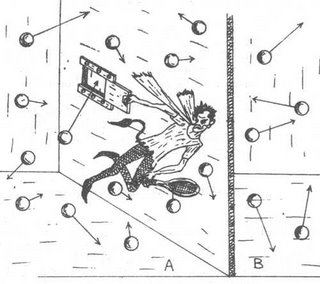
\includegraphics[width=0.6\textwidth]{Figures/MaxwellDemon1.jpg}
\caption{Illustration of Maxwell Demon.(Image taken from\cite{Gamow1940GAMMTI})}
\label{Maxwell}
\end{figure}
The resulting temperature gradient can be used to generate  useful work, which is surprising beacause ideally opening or closing the shutter does not require energy \cite{Gernot}. This violation of the second law of Thermodynamics, has been a subject of discussion for more than one century. The common resolution to the paradox is known as Landauer's principle\cite{5392446}, and its essence is that the missing entropy is generated in the demon's brain during deletion. This also goes along with the dissipation of heat by the demon.\\ 

When this mental experiment was proposed, the technological reality of the time did not allow for a practical understanding of the issue. Nowadays the number of degrees of freedom for systems of interest have significantly decreased and the better controls overs systems have been appeared\cite{PhysRevB.84.245448,cite-key,PhysRevLett.109.180601}. This is the main reason why we bring up the Paradox of Maxwell's demon, as now we can have more control over the systems Maxwell's demon become something more than just an imaginary situation as people had have thought in the past.
\subsection*{Sagawa-Ueda equality.}
After Jarzynski and others developed the classical flutuations theorems, T. Sagawa and M. Ueda generalised again the second law  \cite{PhysRevLett.104.090602,Morikuni2011} for scenarios when the system of interest is subject to feedback control. If the system is tracked under a non equilibrium trajectory, the information obtained in the measurement process can be used to modify the protocol of the external parameters and thus, obtain a different energetic configuration.\\
\begin{equation}
\int P(\{x_i\})e^{-\beta \mathcal{W}(\{x_i\})-I(\{x_i\})}d\{x_i\}=e^{-\beta\Delta F},
\label{Sagawa-Ueda}
\end{equation}
where
\begin{equation}
I(\{x_i\})=\ln\left(\frac{P(y|\{x_i\})}{P(\{x_i\})}\right)
\label{information}
\end{equation}
the information obtained by the measurement outcome $y$. Via Jensen's inequality \eqref{Sagawa-Ueda} yields to
\begin{equation}
\braket{\mathcal{W}}\geq \Delta F - T \braket{I},
\label{secondlaw}
\end{equation}
where $\braket{I}$ corresponds to the mutual information obtained by the feedback control protocol. Equations \eqref{Sagawa-Ueda} and \eqref{secondlaw} generalise the second law in a presence of measurements and feedback. Hence if a feedback cycle is well designed the necessary work to achieve a transition can decrease while for a bad designed protocol the necessary work can take an even upper bound.
\section{Quantum stochastic thermodynamics}
As the system generates work and its environment approach the quantum limit, it becomes increasingly absurd to imagine that they would obey standard thermodynamic rules, since in classical thermodynamics a single particle doesn't have a temperature.
This is one of the reasons why quantum thermodynamics is still not well understood.\\
 At low scales and energy levels of atoms the classical laws of classical physics and its equations of motion failed to describe the results observed in different experiments, thus, the construction of quantum mechanics was made with the purpose of describe this sort of phenomena and its creation completely  changed the way the universe is understood, in particular, regarding the measurement theory\cite{Wiseman}.
\\
Nowadays, the level of control in systems is just astonishing, and due to this he have started to understand different systems which report quantum behaviour, opening then the possibility of machines that change as well the way we interact with nature\cite{0953-8984-18-21-S12,cite-key2}. This new trend of theory and experimental possibilities is know as quantum thermodynamics. However, in order to make a consistent  thermodynamic theory in the quantum mechanical scope, it is necessary to recognise what could change due to the quantum postulates. One of the most challenging questions arises at the main core of the thermochemical  concepts, and this is how to define work and heat?. This is the question  many people have been looking for the answer by using different approaches, nonetheless, it appears that each approach suffers from limitations.
\subsection*{Work is not an observable}
Work is not an observable\cite{PhysRevE.75.050102}. The strong statement seems to exclude the possibility of generalising the laws of thermodynamics to the quantum regime. The main idea behind this statement can be understood by the definition of work.The Hamiltonian $\hat{H}$ appearing in equations \eqref{scrodingereq} and \eqref{liouville-vonnuemann} is the operator associated with the inner energy of the dynamical system. In other words, the average inner energy of the system is 
\begin{equation}
U=\braket{\hat{H}}=\Tr \{\rho\hat{H}\}.
\label{innerenergy}
\end{equation}
The eigenvalues of the Hamiltonian $\hat{H}$ represent the accessible energies for this system. The number of eigenvalues coincide with the dimension $d$ of the Hilbert space. Let's assume that the dynamics evolve from an initial Hamiltonian $\hat{H}_0$ to a final one $\hat{H}_\tau$ with corresponding eigenvalues $E_n$ and $E_m$. Then if a work operator would exist, its possible eigenvalues are all possible combinations $\Delta E_{m,n}=E_m-E_n$\footnote{At the level of individual realisations, thermal and quantum fluctuations make $	Delta U$ a stochastic quantity. The probability distribution $p(u)$ of the total energy change is determined by performing projective measurements $\Pi_m$ and $\Pi_n$, with outcomes $E_n^0$ and $E_m^\tau$ at the beginning and at the end of a driving protocol
\[p(u)=\sum_{m,n}P^{\tau}_{m,n}P^{0}_{n}\delta(u-\Delta E_{m,n}).\] 
 Having an initial and final strong energy measurements as the boundaries of the trajectories justifies the distribution $\delta(u-\Delta E_{m,n})$ for the total change in the inner energy.}.  In the more general case the number of changes in energy can be larger than the dimension $d$ of the Hilbert space. Then there is not an operator in the Hilbert space of the system that can have as many eigenvalues as possible changes in energy.
 \begin{figure}[h]
\centering
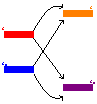
\includegraphics[width=0.6\textwidth]{Figures/energy.pdf}
\caption{Illustration of the possible work values for a 2 dimensional Hilbert Space.}
\label{energy}
\end{figure}
There has been some approach of having a work operator for the case of generalised measurements, which its idea is basically take a larger Hilbert space and create an operator whose eigenvalues correspond to the energy combinations $\Delta E_{m,n}$. Nonetheless, the main message of these two articles is that work is not an observable in the same Hilbert space as the one describing the state of the system $\rho$ or the Hamiltonian $\hat{H}$. With this in mind in next section we are going to provide a manner to formalise quantum thermodynamics via the quantum trajectories and a particular example of POVM which is known as weak measurement\footnote{The advantage of this kind of POVM is that leaves the state almost unperturbed, although tiny information on the system is obtained. Continuous repetition of weak measurements can in practice reproduce an strong measurement.}. Providing us the possibility of measuring quantum trajectories, and via Sagawa-Ueda equality generalise the idea of work and heat at the quantum regime.
\section{Thermodynamics of weakly measured quantum systems.} 
As we mentioned before, thermodynamics is a theory of work and heat with the first and second law as its most important foundations. These laws describe summarise and describe the possible changes in inner energy of a system. For example, a system is know as ``isolated'' if it does not exchange energy with its surroundings through its boundaries. When this conditions is not fulfilled we say that our system is open. Classically, heat is defined as every change in the inner energy that is not work, thus the distinction between work $\mathcal{W}$ and heat $\mathcal{Q}$ depends crucially on the definition of thermal isolation and its possible calculations.\\
Mathematically speaking it is know that the inner energy is an exact differential whereas, work and heat are quantities which are path dependent meaning that are not exact differentials. Translating this in simple words, inner energy depends only on the current state while on the contrary, work and heat do not.
As we will see below we can use the fact that work and heat are quantities which are path dependent since it is possible to use the concept of quantum trajectories to discuss the meaning of work and heat in the quantum regime.\\
The partition of the inner energy  in work and heat established by the first law of thermodynamics also allow us to focus on the deeper insight found in the exchange of energy with its surroundings, in particular we refer to heat. Classically, This quantity is related to the macroscopic definition of the entropy and the reversibility of natural process. For the quantum case, any definition of quantum heat should be in agreement with the current understanding of the second law  and its relation to the entropy should be specified.
\subsection{Quantum work and Heat}
As we mentioned before the idea is to use the fact that work and heat are quantities which are path dependent in order to extend the definition of work and heat for the case of quantum systems at the level of single trajectories. There are mainly two difficulties to identify work and heat at the quantum level. As we mentioned already work is not a quantum observable, which force us to redefine work not as an usual quantum mechanical observable, but as an operation or transformation on the quantum system itself. The second difficulty is related to work path dependence\footnote{It is important to clarify at this point that thermodynamical concepts such as path dependence, isolated system and open system are not in conflict or disagreement with quantum postulates. }. Such constraint raises a challenge as quantum mechanics postulates prevent the tracking of trajectories  without perturbing the system, nonetheless, as we mentioned before this problem can be tackle by using the formalism of weak measurements. If a system is weakly measured the wave function is not collapsed, and then, decoherence do not increase, and the system remains in a superposed quantum state.\\
In order to define work on a quantum system, an isolated system as a gas should be well set and the corresponding changes in the quantum dynamics associated with work. Hence, any change of the Hamiltonian by an external parameter will change the inner energy and this change can be associate only with work if the system is isolated. The evolution for this case is then characterised by a unitary evolution of the Schr\"odinger equation via
\begin{equation}
d\rho_t=-\frac{i}{\hbar}[\hat{H}_t,\rho_t]dt=\mathbb{W}[\rho_t]dt,
\label{Work}
\end{equation}
where the we have defined ``work''\footnote{This is not exactly the classical definition of work, so its important to do not confuse them, here the super-operator of work is defined in order to make use of quantum trajectories and generalise the concept of work at quantum level. } as a super-operator $\mathbb{W}[\rho_t]=-i/\hbar [\hat{H}_t,\rho_t]$ and its time dependency it's explicit. \\
The dynamical evolution of the system given by Scr\"odinger equation defines an unitary evolution operator 
\begin{equation}
\hat{\mathcal{U}}=\hat{\mathcal{T}}\text{exp}\left(-\frac{i}{\hbar}\int \hat{H}_t dt'\right),
\label{Unitaryevolution}
\end{equation}
where $\hat{\mathcal{T}}$ is the time ordering operator.\\
As we mentioned before work can not be an operator, nonetheless, here work was identified as the unitary transformation \eqref{Unitaryevolution} done upon the state of the system $\rho_t$\cite{2540650509c442d0b14e917fdf7a4ca7}. This assignation provide us several features. First applying the concept of unitary transformation to the density matrix, the definition of quantum observables is no longer required which results in agreement with the work presented in\cite{PhysRevE.75.050102}\footnote{An other aspect of the definition is that an understanding of transformations done upon the system is assumed, which means that we are able to keep track the dynamics of the system, which henceforth will be called trajectory. Such trajectory dependence is in full agreement with the classical definition of work, and what we are suggesting here is that we do not expect it to be much different since the is no disagreement between a quantity to be path dependent and the postulates of quantum mechanics.}.
\subsection{Open system}
Let's imagine a system which has the possibility to exchange energy with its surroundings. Here we suppose that the work was previously calculated for the isolated case, therefore, the additional possible changes in the inner energy should be associated with the a new quantity ``Heat''.\\
In the case of quantum levels, nothing forbid us to think as in the classical case. Once work is defined for an isolated system such as we did in \eqref{Work}, the natural stage to follow is to open the system to possible interactions with its surroundings ans associate everything which is not work with a new form of energy change
\begin{align}
\mathbb{Q}[\rho_t]dt&=d\rho_t -\mathbb{W}[\rho_t]dt\nonumber\\
d\rho_t&=\mathbb{W}[\rho_t]dt+\mathbb{Q}[\rho_t]dt,
\label{firstLaw}
\end{align}
which states the equivalent to the first law of quantum thermodynamics.\\
Hence, the evolution of the density operator is divided into two contributions. The first contribution is associate with work, and this corresponds to the unitary evolution due to the Hamiltonian driving of the quantum system. The second contribution is in simple term, what is left, and this corresponds to the non unitary part. Therefore, equation \eqref{firstLaw} generalise the first law of thermodynamics in the quantum realm. It should not be surprising since in classical dynamics the energy contains all the thermodynamic information of the system, the quantum quantity which summarise the full dynamics, time evolution, coherence and probabilistic behaviour, is the density matrix $\rho$.\\
Notice that the definitions of work and heat provide before in \eqref{firstLaw} and \eqref{Work} are in agreement with averages quantities. At the ensamble level, it is possible to see that quantum work and heat are introduced by considering an infinitesimal variation of the mean energy, $U=\braket{\hat{H}}=\Tr(\rho_t\hat{H}_t)$, recovering then the classical stochastic result which extend the firs law to a single realisation of the stochastic outcome.
\begin{align}
dU&=\Tr(\rho d\hat{H})+\Tr (d\rho \hat{H})\nonumber\\
&=\Tr(\rho d\hat{H})+\Tr(\hat{H}\mathbb{W}[\rho]dt)+\Tr(\hat{H}\mathbb{Q}[\rho]dt)\nonumber\\
&=\Tr(\rho d\hat{H})+\Tr(\hat{H}\mathbb{Q}[\rho]dt)\nonumber\\
&=\delta W + \delta Q.
\label{reductionfirstlaw}
\end{align}
Note that the association of work with an unitary process leads to an averaged null work super-operator contribution
\begin{equation}
\Tr(\hat{H}\mathbb{W}[\rho]dt)=\frac{i}{\hbar}\Tr(\hat{H}[\rho,\hat{H}])dt=0.
\end{equation}
Which is expected, due to the fact that changes in the inner energy due to an unitary evolution are encoded in the Hamiltonian. Thus, by averaging over quantum fluctuations we arrive to the stochastic version of the first law of thermodynamics.\\
On the other hand the heat appears to be fundamentally associated with the non unitary part of the dynamics, and as we saw in the first chapter, in the general case an open system can be described by what is known as the quantum master equation. Hence, the Lindblad master equation is in agreement with the given description in chapter one. This leads us to the conclusion that there is not an unitary transformation which can be associate with heat, how ever it seems plausible to extract the information about work and heat at quantum level.\\
with this in mind and motivated by the experiments presented in \cite{experiment1,experiment2}, we will show how the concepts we presented above can be used in order to calculate the thermodynamic quantities for the case of a monitored  qubit.
\section{Application to a monitored quibit.}
In order to implement the formalism we presented in the previous section, we consider a driven two level system $S$ witha time-dependent Hamiltonian given by.
\begin{equation}
\hat{H}_{S}=\epsilon\hat{\sigma}_z+\lambda_t \hat{\sigma}_x,
\label{Hamiltonianqbit}
\end{equation}
where $\lambda_t$ is the external driving which functional form will be specified later, and $\hat{\sigma}_i$ are the Pauli matrices. The evolution described by \eqref{Hamiltonianqbit} induces an unitary evolution on the qubit, which will be associated with work since the dynamics is consider isolated. The system is continuously   coupled to a detector $D$ via the interaction of the Hamiltonian $\hat{H}_{I}$, then the total Hamiltonian can be written as
\begin{equation}
\hat{H}_T=\hat{H}_{S}+\hat{H}_{D}+\hat{\sigma}_z\hat{H}_{I},
\label{Totalhamiltonian}
\end{equation}
where, the system is coupled to the detector by the observable $\hat{\sigma}_z$. The effects of the detector is characterised by the averaged signals, $(I_1,I_2)$, and Gaussian noises $(S_1,S_2)$, measured when the qubit is in two eigenstates $(\ket{0},\ket{1})$, of the measured observable. Here is assumed that the detector is weakly coupled to the detector and then we have that signal which distinguish state $\ket{0}$ from $\ket{1}$, $(\Delta I=I_2-I_1)$ is much weaker than the typical signal $(I_0=(I_1+I_2)/2)$. The measurement time $\tau_M=(S_1+S_2)/(I_1-I_2)^2$ sets the time scale of after which the detector clearly distinguish the state $\ket{0}$ from $\ket{1}$ and hence performs a projective measurement.\cite{2540650509c442d0b14e917fdf7a4ca7}\\
The qubit described by the Hamiltonian \eqref{Totalhamiltonian} is interpreted to be a double quantum dot sharing a single electron and interacting with a quantum point contact. Identifying the configurations where the electron occupies only one dot ($\braket{\sigma_z}=\pm 1$)\footnote{Also Coherent superposition of the two states are possible.}. The detector which monitor the occupation of the dots is a voltage biased given by the quantum point contact (QPC) with Hamiltonian \cite{PhysRevB.56.15215,PhysRevB.63.115403,Alexander}
\begin{equation}
\hat{H}_D=\sum_l \epsilon_l \hat{c}_{l}^{\dagger}\hat{c}_l+\sum_r \epsilon_r \hat{c}_{r}^{\dagger}\hat{c}_{r}+\sum_{r,l} \Omega (\hat{c}_{r}^{\dagger}\hat{c}_{l}+\hat{c}_{l}^{\dagger}\hat{c}_{r}),
\label{detectorhamiltonian}
\end{equation}
and the Hamiltonian of the interaction given by
\begin{equation}
\hat{H}_{I}=\sum_{r,l}\frac{\delta \Omega}{2}(\hat{c}_{r}^{\dagger}\hat{c}_{l}+\hat{c}_{l}^{\dagger}\hat{c}_{r}).
\label{interactionHamiltonian}
\end{equation}

The output signal we can record from the detector is given by the current $I(t)$ across the QPC, with averages $I_{1(2)}=2\pi\Omega_{1(2)}^{2}\rho_l\rho_r e^{2} V /\hbar=e^{2}T_{1(2)}V/\hbar$ and noises $S_{1(2)}=e(1-T_{1(2)})$, where $\rho_{l,r}$ are the densities of states in the left and the right electrodes, and $T_{1(2)}$ are the transition probabilities across QPC.
\subsection{Equation of motion.}
Given the Hamiltonian of the system is it possible to compute the equations of motion of our system we can make use of the equation \eqref{Itolindbladeq} by assuming that the system is coupled to a dephasing bath, therefore $\hat{J}\propto \hat{\sigma}_z$ as suggested in \cite{PhysRevB.56.15215}. Therefore computing each term in equation \eqref{Itolindbladeq} by setting $\hat{J}=\frac{\Delta I}{2\sqrt{2S_0}}\hat{\sigma}_z=\sqrt{\gamma}\hat{\sigma}_{z}$\footnote{Where $\Delta I=I_{2}-I_1$}, with $\sqrt{\gamma}=\frac{\Delta I}{2\sqrt{2S_0}}$\footnote{Here we consider the noise $d\xi$ to be real, $d\xi^{*}=d\xi$}
\begin{equation}
[\hat{H},\rho]=\begin{pmatrix}
\lambda_t(\rho_{21}-\rho_{12}) & 2\epsilon\rho_{12}+\lambda_t(\rho_{22}-\rho_{11})\\
\lambda_t(\rho_{11}-\rho_{22})-2\epsilon\rho_{21} & \lambda_t(\rho_{12}-\rho_{21}) 
\end{pmatrix},
\label{first}
\end{equation}
\begin{equation}
\mathcal{L}[\hat{J}]=\begin{pmatrix}
0 & -2\gamma \rho_{12}\\
-2\gamma\rho_{21} & 0
\end{pmatrix},
\label{second}
\end{equation}
\begin{align}
&(\hat{J}-\braket{J})\rho d\xi^{*}+\rho(\hat{J}^{\dagger}-\braket{J}^{\dagger})d\xi=\nonumber\\
&\begin{pmatrix}
-2\sqrt{\gamma}(\rho_{11}-\rho_{22}-1)\rho_{11} & -2\sqrt{\gamma}\rho_{21}(\rho_{11}-\rho_{22})\\
-2\sqrt{\gamma}(\rho_{11}-\rho_{22})\rho_{21} & -2\sqrt{\gamma}\rho_{22}(1+\rho_{11}-\rho_{22})
\end{pmatrix}d\xi.
\label{third}
\end{align}
Therefore, putting the equations \eqref{first}, \eqref{second} and \eqref{third} all together, this leads us to the equations of motion:
\begin{equation}
d\rho_{11}=-2\frac{\lambda_t}{\hbar}\Im\text{m}(\rho_{12})dt+2\frac{\Delta I}{\sqrt{2S_{0}}}\rho_{11}(1-\rho_{11})d\xi,
\label{motioneq1}
\end{equation}
\begin{equation}
d\rho_{12}=-2i\frac{\epsilon}{\hbar}\rho_{12}dt-\frac{i}{\hbar}\lambda_t(1-2\rho_{11})dt -\rho_{12}\frac{\Delta I^{2}}{4S_{0}}dt+2\frac{\Delta I}{\sqrt{2S_{0}}}(1-2\rho_{11})\rho_{12}d\xi.
\label{motioneq2}
\end{equation}
However, we notice that, the term $\frac{\Delta I^{2}}{4S_{0}}$ has units of inverse time, so it is possible to redefine the noise
\[\sqrt{\frac{S_0}{2}}\xi=d\xi,\]
by doing this we have that equations \eqref{motioneq1} \eqref{motioneq2} can be written in the Îto's form\footnote{Here $\Im\text{m}$ symbolise the imaginary part.}
\begin{equation}
d\rho_{11}=\left(-2\frac{\lambda_t}{\hbar}\Im\text{m}(\rho_{12}))\right)dt+\frac{2\Delta I}{S_0}\rho_{11}(1-\rho_{11})\xi(t),
\label{rho11}
\end{equation}
\begin{equation}
d\rho_{12}=\left(-2i\frac{\epsilon}{\hbar}\rho_{12}-\frac{i}{\hbar}\lambda_t(1-2\rho_{11})-\frac{\Delta I^2}{4S_0}\rho_{12}\right)dt+\frac{\Delta I}{S_0}\rho_{12}(1-2\rho_{11})\xi(t),
\label{rho22}
\end{equation}
which coincide with equation in \cite{PhysRevB.63.115403,Alexander,2540650509c442d0b14e917fdf7a4ca7} for the case of perfect detection.\\
Computing now the detector current by using equation \eqref{current} we obtain that:
\begin{align*}
Y dt&=dt\braket{u\hat{J}^{\dagger}+\hat{J}}+d\xi\\
&=dt(u+1)\braket{\hat{J}}+d\xi\\
&=\sqrt{\gamma} dt (u+1)(\rho_{11}-\rho_{22})+d\xi\\
&=\frac{\Delta I}{2\sqrt{2S_0}}(u+1)(2\rho_{11}-1)+d\xi.
\end{align*}
Therefore, associating the current calculated above with the output of the detector via 
\[Ydt=\sqrt{\frac{2}{S_0}}(I(t)-I_0).\]
Leading us to
\[I(t)=I_0+\frac{\Delta I}{4}(u+1)(2\rho_{11}-1)+\sqrt{\frac{S_0}{2}}d\xi.\]
Setting $u=1$, meaning that the protocol of detection is an Homodyne\cite{WISEMAN200191}, leads us to the equation given in \cite{2540650509c442d0b14e917fdf7a4ca7}\footnote{Remembering that $u$ give us the correlation in the noise, it is important to emphasise that depending on the protocol the noise we are working with could be correlated.}.
\begin{equation}
I(t)=I_0 + \frac{\Delta I}{2}(2\rho_{11}-1)+\xi(t).
\label{currentqbit}
\end{equation}
This is an experiment proposed in \cite{2540650509c442d0b14e917fdf7a4ca7}, at it is specially interesting since the equations of motion \eqref{rho11} and \eqref{rho22} allow to identify the  unitary and non unitary contributions to the time evolution, because these two equations can be written in the fashion of \eqref{firstLaw}
\[d\rho_t=\delta\mathbb{W}[\rho_t]dt+\frac{\Delta I}{S_0}\delta\mathbb{M}[\rho_t]dt.\]
By expressing the first law of quantum thermodynamics, particularly for this case, the non unitary part (Heat) becomes accessible since it is proportional to the signal of the detector $\Delta I$, which is interpreted as the heat associated with the detector back action ($\delta\mathbb{Q}=(\Delta I /S_0)\delta\mathbb{M}$). The factor $\delta\mathbb{W}$ is identified as the work done by the driving $\lambda_t$ along an infinitesimal trajectory\footnote{Note that equation \eqref{reductionfirstlaw} tell us that if the Hamiltonian is time independent, then the system doesn't make any work since $dH_{t}=0$ and then the change of inner energy in the system is given only by the changes of heat.}.\\
As the equations of motion \eqref{rho11} and \eqref{rho22} are  nonlinear stochastic master equations, the way of have knowledge about the contributions due to the work and heat has to determined numerically.
 
\section{Solving the equation}
In order to solve the equations \eqref{rho11} and \eqref{rho22} we specify the the driving, defining it as  $\lambda_t=g(1/\cosh(\nu(1-t/\tau)))$ where $\tau$ is the duration of the experiment. 
\begin{figure}[h]
\centering
\includegraphics[width=0.7\textwidth]{../Program/driving/drive.pdf}
\caption{External driving of the Hamiltonian for $g=1$, $\tau=10$ and $\nu=8$. As we can appreciate in this figure, the behaviour of the driving is almost naught for more than the half of the time of the experiment, while for the rest of the experiment faster changes occur due to the driving.}
\label{driving}
\end{figure}
Therefore, it is possible to solve the equations of motion via a numerical method, here we use the method called \textit{order 2.0 weak Runge-Kutta scheme} proposed by Platen \cite{Kloeden1992}, by generating Wiener increments ($dW$) with mean zero and variance $dt=0.01$, we make this for $300$ realisations.\\
the evolution of the system in the time interval $[0,\tau]$ along an individual quantum trajectory $\rho_t$ can be divided into $N=\tau/dt$ successive infinitesimal unitary steps $\mathcal{U}_{i}$ generated by the Hamiltonian and other $N$ quantity of non-unitary steps $\mathcal{N}_i$ due to the coupling with the detector\footnote{Here we chose just by convenience the unitary and non-unitary processes to correspond to the odd and even steps respectably}.
\begin{align}
\rho_0\xrightarrow{\mathcal{U}_1}\rho_1\xrightarrow{\mathcal{N}_2}\rho_{2}\ldots\nonumber\\
\ldots\rho_{2i-2}\xrightarrow{\mathcal{U}_i}\rho_{2i-1}\xrightarrow{\mathcal{N}_i}\rho_{2i}\ldots\nonumber\\
\ldots\rho_{2N-2}\xrightarrow{\mathcal{U}_N}\rho_{2N-1}\xrightarrow{\mathcal{N}_N}\rho_{2N}.
\end{align}
Thus, each transformation induces a change in the state of the system defined as,
\begin{equation}
\delta\mathbb{W}[\rho_{i}]dt=\rho_{2i-1}-\rho_{2i-2},
\label{changeofwork}
\end{equation} 
\begin{equation}
\delta\mathbb{Q}[\rho_{i}]dt=\rho_{2i}-\rho_{2i-1}.
\label{changeofheat}
\end{equation}
As we said before $d\rho$ is supposed to be an exact differential, meaning that this is path independent, then the total change of the density operator can then be written as
\[
d\rho=\rho_{2N}-\rho_{0}
\]
\[
=\underbrace{\rho_{2N}-\rho_{2N-1}}_{\delta\mathbb{Q}[\rho_{N}]dt}+\underbrace{\rho_{2N-1}-\rho_{2N-2}}_{\delta\mathbb{W}[\rho_{N}]dt}+\ldots+\underbrace{\rho_{2}-\rho_{1}}_{\delta\mathbb{Q}[\rho_1]dt}+\underbrace{\rho_{1}-\rho_{0}}_{\delta\mathbb{W}[\rho_{1}]dt}
\]
\begin{equation}
=\sum_{i=1}^{N}\delta\mathbb{W}[\rho_{i}]dt+\sum_{i=1}^{N}\delta\mathbb{Q}[\rho_{i}]dt.
\label{Contributions}
\end{equation}
Meaning that with equation \eqref{Contributions} is is possible to distinguish between the unitary (work) and non unitary (heat) contributions to the final state. Notice that just in the case when the density matrix $\rho$ is used to evaluate the energy change, the distinction between unitary and non unitary transformations take an energetic character.
\section{Results}
Up to this point, the formulation of the laws of thermodynamics has been defined in the quantum realm, and the separation of the unitary and the non-unitary contributions in the equation of motion for the density matrix allow us to calculate the dynamical quantities for our specific example of a qubit coupled to a quantum detector.\\
At the level of a quantum trajectory it is possible to calculate the stochastic contributions for work, heat and energy in equation \eqref{reductionfirstlaw}. \\
In figure \ref{qbitenergy} we present the result of tracing along a single trajectory in order to identify the contributions of  work ($\delta W$), heat($\delta Q$) and energy ($dU$).As we expected the heat and work contributions give us the contribution in energy, meaning that the first law is confirmed for the qubit system. From figure \ref{qbitenergy} we see that the heat contribution is clearly visible, confirming the fact that our system is not isolated.\\
From the experimental point of view, the current we compute $Ydt$ presented in figure \ref{qbitcurrentfig} can be measured, since this current corresponds to the Fourier transform of the output $I(t)$, therefore, by measuring this current it is possible to reconstruct the quantum state of the system by using \eqref{rho11}, \eqref{rho22},\eqref{currentqbit} and the known driving  $\lambda_t$, giving us an alternative to reconstruct states and identify experimentally work and heat contributions along single quantum trajectories. \\
\begin{figure}[h!]
\centering
\includegraphics[width=0.9\textwidth]{../Program/Thermodynamics/Energy.pdf}
\caption{Infinitesimal change of work, heat and energy along a single quantum trajectory. The parameters used were $\epsilon=1$ , $\hbar=1$, $\gamma=5\cdot 10^{-3}$, $g=6.25$, $\tau=3$ and $\nu=8$. For each realisation the initial state was the ground state.}
\label{qbitenergy}
\end{figure}
\begin{figure}[h!]
\centering
\includegraphics[width=0.9\textwidth]{../Program/Thermodynamics/Current.pdf}
\caption{Corresponding current signal $Ydt$ in the detector.}
\label{qbitcurrentfig}
\end{figure}
In figure \ref{Blocksphere} we show the temporal evolution of the qubit over the Block sphere, as we can see the qubit is initially in the ground state, and due to the driving the state of the qubit start to change, however, as one can appreciate there is no significant change between the average over trajectories and a single trajectory. Once we have solved equations \eqref{rho11} and \eqref{rho22} numerically we are able to compute quantities such as the inner energy.\\
In figure \ref{innerenergy} we show the behaviour of the inner energy, which has the behaviour that we expected since the driving start to increase making evolve the energy as
\[U(t)\xrightarrow[t\rightarrow \tau]{}\braket{\hat{\sigma}_x}\lambda_t.\]
\begin{figure}[h!]
\centering
\includegraphics[width=1.0\textwidth]{../Program/Thermodynamics/Bloschsphere.pdf}
\caption{Temporal evolution of the qubit over the Block sphere. Each plot has two curves which correspond to an average over 100 trajectories and a single trajectory.}
\label{Blocksphere}
\end{figure}
\begin{figure}[h!]
\centering
\includegraphics[width=0.8\textwidth]{../Program/Thermodynamics/Innerenergy.pdf}
\caption{Inner energy of the qubit as a function of time.}
\label{qbitinnerenergy}
\end{figure}
\chapter*{Conclusions}
We first started discussing about how open quantum systems were treated and how it is possible to determine the dynamics of a system via a master equation.\\
Then in the second part used formalism of quantum trajectories in order to generalise the Schr\"odinger equation into a stochastic master equation for a state conditioned to continous measurements. This lead us to the diffusive unravelings which allowed us to find quantities such as the currents which characterised the measuring.
Finally we took all this concepts in order to provide an extension of the first law of stochastic thermodynamics along individual trajectories by using an special kind of POVM named weak measurement. By doing this we showed that it is possible to distinguish quantities associated with the unitary and non-unitary transformations done on the density matrix which we associated with work and heat respectively at the quantum level.
We also attested that by doing this association it is possible to recover the results of stochastic thermodynamics.\\
As an application we took a model of a qubit coupled by a dephasing bath, finding that for this example it is possible to distinguish the heat and work in the qubit by measuring the output of the quantum detector, letting us also to reconstruct the state of the system.
